\chapter{伺服器架構}
\renewcommand{\baselinestretch}{10} %設定行距
%\section{前言}
\par
\renewcommand{\baselinestretch}{1} %設定行距
\twelve \qquad 此專題採用Windows 10版本作為我們的架設所使用作業系統,Windows作業系統在作業系統中的市佔率高達七成五以上,且Windows 10作業系統在Windows作業系統中的使用率高達八成以上。
\\
\par
\renewcommand{\baselinestretch}{1} %設定行距
\twelve \hspace{0.5em} 以下為Windows作業系統與Linux作業系統的比較。
\par
\\
\begin{center}
\begin{tabular}{|l|p{6.5cm}|p{6.5cm}|} %表格
\hline
比較&Windows&Linux 
\\
\hline
介面&介面統一,所有Windows程式選單幾乎一致。&圖形介面風格依發行版不同而不同,可能互不相容。
\\
\hline
使用&使用比較簡單,容易入門。圖形化介面對沒有電腦背景知識的使用者使用十分有利&命令列介面,需要學習才能掌握,但也有圖形介面使用上,也較令另列易上手。
\\
\hline
學習&系統構造複雜、變化頻繁,且知識、技能淘汰快,深入學習困難。&系統構造簡單、穩定,且知識、技能傳承性好,深入學習相對容易。
\\
\hline
軟體&商業軟體為主。有很多軟體只能在windows裏運行,無法相容Linux。&自由軟體為主。Linux相容的軟體有需多處於開發中,選擇性相對Windows較少。
\\
\hline
使用者&七成五以上。&不到一成。
\\
\hline
\end{tabular}
\end{center}

\renewcommand{\baselinestretch}{20} %設定行距
\section{Windows 環境配置}
\par
\renewcommand{\baselinestretch}{1} %設定行距
\twelve \qquad 在Window系統安裝完成後,將所需要的軟體安裝到系統上,之後將安裝的軟體在系統上設定環境變數。
\\
\par
\renewcommand{\baselinestretch}{1} %設定行距
\twelve \hspace{0.5em} 環境變數是一個動態命名的值,可以影響電腦上行程的行為方式,使用者通過設定環境變數,來更好的執行程序。
\\
\par
\renewcommand{\baselinestretch}{1} %設定行距
\twelve \hspace{0.5em} 在作業系統搜尋如(圖\ref{fig.關鍵字})
\\
\par
\renewcommand{\baselinestretch}{1.7} %設定行距
\begin{figure}[hbt!]
\begin{center}

\includegraphics[width=3in]{5}
\caption{\large 關鍵字}\label{fig.關鍵字}
\end{center}
\end{figure}
\par
\\
\renewcommand{\baselinestretch}{1} %設定行距
\twelve \hspace{0.5em} 選擇環境變數如(圖\ref{fig.環境變數})
\\
\par
\renewcommand{\baselinestretch}{1.7} %設定行距
\begin{figure}[hbt!]
\begin{center}
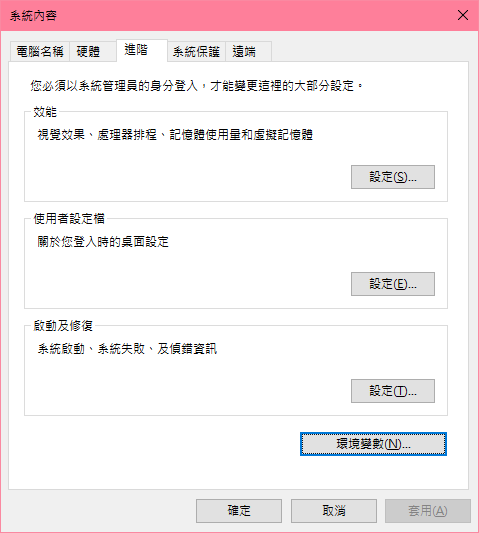
\includegraphics[width=5in]{6}
\caption{\large 環境變數}\label{fig.環境變數}
\end{center}
\end{figure}
\par
\\
\renewcommand{\baselinestretch}{1} %設定行距
\twelve \hspace{0.5em} 選擇系統變數中的Path如(圖\ref{fig.Path})
\\
\par
\renewcommand{\baselinestretch}{1.7} %設定行距
\begin{figure}[hbt!]
\begin{center}
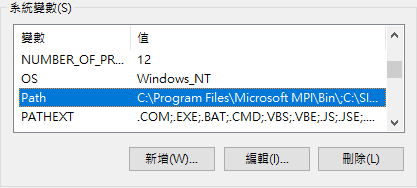
\includegraphics[width=4in]{7}
\caption{\large Path}\label{fig.Path}
\end{center}
\end{figure}
\par
\\
\renewcommand{\baselinestretch}{1} %設定行距
\twelve \hspace{0.5em} 新增變數並且指定路徑如(圖\ref{fig.編輯環境變數})
\\
\par
\renewcommand{\baselinestretch}{1.7} %設定行距
\begin{figure}[hbt!]
\begin{center}
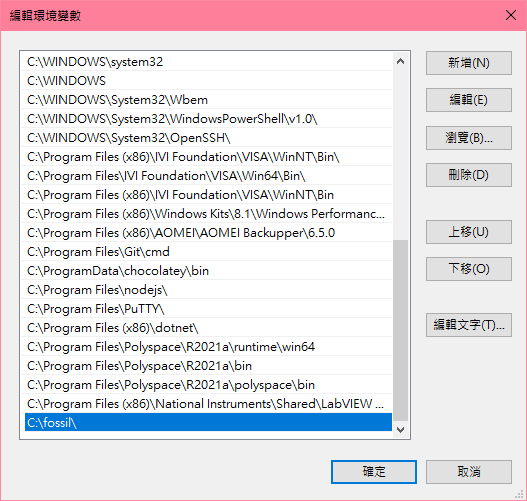
\includegraphics[width=5in]{8}
\caption{\large 編輯環境變數}\label{fig.編輯環境變數}
\end{center}
\end{figure}
\par

\renewcommand{\baselinestretch}{20} %設定行距
\section{Fossil SCM}
\par
\renewcommand{\baselinestretch}{1} %設定行距
\twelve \qquad 對於研究或專案計畫而言,工作中經常使用的具是電腦或其他相關電子產品,而對於研究過程或開發的流程、錯誤及解果的每個步驟都相刀的重要,而對負責軟體開發工作的軟體團隊成員來說,版本控制系統是一套相當重要的軟體工具。如果沒有版本控制系統,開發團隊成員將難以有效控制研究或開發過程,並可能導致效率的增加。
\\
\par
\renewcommand{\baselinestretch}{1} %設定行距
\twelve \hspace{0.5em} 目前已經存在許多成熟的版本控制系統,例如較為知名的 Git、Subversion或CVS等等。若以架設方式加以細分,則有分散式與Client-Server二種不同的系統分類。除了這些系統以外,網路上還可以找到許多其他各具特色的版本控制系統。雖然這些系統的知名度較低,但如果仔細檢視其優點與特色,仍然可以找到一些頗為出色的版本控制系統。
\\
\par
\renewcommand{\baselinestretch}{1} %設定行距
\twelve \hspace{0.5em} 因此本專題所使用的是Fossil,是一套採用分散式處理方式的版本控制系統。
\\
\par
\renewcommand{\baselinestretch}{1.7} %設定行距
\begin{figure}[hbt!]
\begin{center}

\includegraphics[width=1in]{9}
\caption{\large Fossil}\label{fig.Fossil}
\end{center}
\end{figure}
\par
\\
\renewcommand{\baselinestretch}{1} %設定行距
\twelve \hspace{0.5em} 因此本專題所使用的是Fossil,是一套採用分散式處理方式的版本控制系統。
\par

\renewcommand{\baselinestretch}{20} %設定行距
\subsection{特色}
\par
\renewcommand{\baselinestretch}{1} %設定行距
\twelve \qquad 一般人對於軟體本身的使用需求,多半是希望越容易操作越好,並且有相當程度的穩定性與可靠性。而操作簡單與系統本身穩定性高,正是Fossil所強調的二大重點。
\\
\par
\renewcommand{\baselinestretch}{1} %設定行距
\twelve \hspace{0.5em} 在穩定性方面,Fossil採用SQLite資料庫作為儲存的平台,再加上永久性的檔案結構,即使遭遇斷電或是元件(不包括硬碟)損毀等問題,資料也不會損失。
\\
\par
\renewcommand{\baselinestretch}{1} %設定行距
\twelve \hspace{0.5em} 在可靠性方面,Fossil目前也正在研發新的保護機制,在未來的版本中將會提供自動檢查機制,只要資料提交,系統便會自動進行資料內容驗證,以確保資料內容無誤,以提升可靠性。
\\
\par
\\
\renewcommand{\baselinestretch}{1} %設定行距
\twelve \hspace{0.5em} Fossil之所以可以作為官方網站的平台,是因為除了版本控制系統相關的功能以外,亦可利用Fossil作為Blog 平台的架設方案。所以無論使用者需要的是單純的版本控制,或是希望架設網站作為資訊分享的平台,都能利用Fossil一併解決。所以在取得Fossil之後,不只獲得Fossil本身的原始碼,還取得了一整個網站系統的架設方案。
\par
\\

\renewcommand{\baselinestretch}{20} %設定行距
\subsection{功能}
\par
\renewcommand{\baselinestretch}{1} %設定行距
\begin{enumerate}
	\item \textbf{項目管理:} 除了像Git和Mercurial那樣做分佈式版本控制之外,Fossil還支持錯誤追蹤、wiki、論壇、電子郵件警報、聊天和技術說明。
	\item \textbf{Web介面:} Fossil具有內置、主題化、可擴展和直觀的Web界面,其中包含豐富多樣的信息頁面。
	\item \textbf{一體式:} Fossil是一個獨立的、獨立的可執行文件。要安裝,只需下載適用於Linux、Mac或Windows的預編譯二進製文件,並將其放在PATH上。還提供易於編譯的源代碼。
	\item \textbf{自託管:} 使用各種技術在幾分鐘內建立一個項目網站。Fossil具有CPU和內存效率。大多數項目可以舒適地託管在每月5美元的VPS 或Raspberry Pi上。還可以設置自動GitHub鏡像。
	\item \textbf{簡單網路系統:} Fossil使用普通的HTTPS或SSH進行網絡通信,因此它可以在防火牆和代理後面正常工作。該協議帶寬效率很高,以至於Fossil可以通過撥號、弱3G或客機Wifi輕鬆使用。
	\item \textbf{自動同步:} Fossil支持自動同步模式,通過減少與分佈式項目相​​關的不必要的分叉和合併數量,有助於保持項目向前發展。
	\item \textbf{開源:} BSD授權條款。
\end{enumerate}
\par

\renewcommand{\baselinestretch}{20} %設定行距
\subsection{Fossil 操作簡介}
\par
\renewcommand{\baselinestretch}{1} %設定行距
\twelve \qquad Fossil與其他版本控制系統相同,主要使用的都是儲存庫(Repository)的概念。儲存庫可以視為一種資料庫,其中存放了專案相關的檔案與資料等等。使用者處理這些檔案時,需要先將資料取出(Check Out)並存放至本地端中,也就是使用者的工作目錄。等到完成了新增、修改等各種工作,再將本地端的資料回存(Check In)至儲存庫之中,即可完成整個處理作業。也就是說,在使用Fossil時,主要的動作有三項:新增或複製儲藏庫、取出資料、進行資料處理與存取等工作。
\\
\par
\renewcommand{\baselinestretch}{1} %設定行距
\twelve \hspace{0.5em} 專ㄋ案開始執行時,需要新增一個儲藏庫,此時可以使用下列指令,建立一個新的儲存庫。儲存庫名稱未限制,因此可以使用任何命名方式,也可以不用使用任何副檔名。
\par
\begin{center}
\begin{tabular}{||p{15cm}|} %表格
\hline
\textbf{fossil init} \emph{repository-filename}
\\
\hline
\end{tabular}
\end{center}
\par
\renewcommand{\baselinestretch}{1} %設定行距
\twelve \hspace{0.5em} 儲存庫是以檔案方式存在於系統之中,所以執行此指令之後,便可在檔案系統中找到以儲存庫名稱命名的檔案。大多數Fossil的操作都針對本地的儲存庫進行處理,如果需要存取遠端系統中的儲存庫,以下列指令將遠端儲存庫複製到本地中,再進行後續處理。
\par
\begin{center}
\begin{tabular}{||p{15cm}|} %表格
\hline
\textbf{fossil clone} \emph{https://your-id-num@your-domain-name/ your-db.fossil}
\\
\hline
\end{tabular}
\end{center}
\par
\renewcommand{\baselinestretch}{1} %設定行距
\twelve \hspace{0.5em} 建立或複製完儲存庫之後,此時可以先建立一個新目錄,切換到此目錄並且以下列指令展開取得\_ FOSSIL\_ 檔案。
\par
\begin{center}
\begin{tabular}{||p{15cm}|} %表格
\hline
\textbf{fossil open} \emph{repository-filename}
\\
\hline
\end{tabular}
\end{center}
\par
\renewcommand{\baselinestretch}{1} %設定行距
\twelve \hspace{0.5em} 此時可以將所需提交的檔案放置此目錄,並且以下列指令將指定的檔案加入到儲存庫。
\par
\begin{center}
\begin{tabular}{||p{15cm}|} %表格
\hline
\textbf{fossil add} \emph{file...}
\\
\hline
\end{tabular}
\end{center}
\par
\renewcommand{\baselinestretch}{1} %設定行距
\twelve \hspace{0.5em} 若需要儲存庫的資料刪除,以下列指令將指定的檔案刪除於儲存庫。
\par
\begin{center}
\begin{tabular}{||p{15cm}|} %表格
\hline
\textbf{fossil rm} \emph{file...}
\\
\hline
\end{tabular}
\end{center}
\par
\renewcommand{\baselinestretch}{1} %設定行距
\twelve \hspace{0.5em} 如果覺得依序加入或移除檔案的方式有些麻煩,則可以以下列指令,讓儲存庫與本地目錄中的檔案清單自動的做對比,如果有檔案存在於本地目錄,但並未在儲存庫之中出現,則會自動將此檔案加入儲存庫之中。相反的,如果檔案只出現在儲存庫,但本地目錄中找不到該檔案,則會自動將此檔案自儲存庫之中移除。
\par
\begin{center}
\begin{tabular}{||p{15cm}|} %表格
\hline
\textbf{fossil addremove}
\\
\hline
\end{tabular}
\end{center}
\par
\renewcommand{\baselinestretch}{1} %設定行距
\twelve \hspace{0.5em} 當新增或刪除的部分完成時,需要以下列指令做最後的提交,所新增或刪除的檔案才會正式生效。
\par
\begin{center}
\begin{tabular}{||p{15cm}|} %表格
\hline
\textbf{fossil commit}
\\
\hline
\end{tabular}
\end{center}
\par
\renewcommand{\baselinestretch}{1} %設定行距
\twelve \hspace{0.5em} 以上僅是Fossil最基本的操作方式,並未完整涵蓋Fossil所有的指令與其參數。以下為Fossil經常使用的指令。
\\
\par
\begin{center}
\begin{tabular}{|p{2cm}|p{2cm}|p{2cm}|p{2cm}|p{2cm}|p{2cm}|} %表格
\hline
add          &cat          &diff         &ls           &remote       &tag
\\
\hline
addremove    &changes      &extras       &merge        &revert       &timeline
\\
\hline
all          &chat         &finfo        &mv           &rm           &ui
\\
\hline
amend        &clean        &gdiff        &open         &settings     &undo
\\
\hline
annotate     &clone        &grep         &patch        &sql          &unversioned
\\
\hline
bisect       &commit       &help         &pull         &stash        &update
\\
\hline
blame        &dbstat       &info         &push         &status       &version
\\
\hline
branch       &delete       &init         &rebuild      &sync         &xdiff
\\
\hline
\end{tabular}
\end{center}

\clearpage %換頁
\renewcommand{\baselinestretch}{20} %設定行距
\section{Stunnel}
\par
\renewcommand{\baselinestretch}{1} %設定行距
\twelve \qquad Stunnel是一種代理,旨在將TLS加密功能添加到現有客戶端和服務器,而無需對程序代碼進行任何更改。 它的架構針對安全性、可移植性和可擴展性(包括負載平衡)進行了優化,使其適用於大型部署。
\\
\par
\renewcommand{\baselinestretch}{1.7} %設定行距
\begin{figure}[hbt!]
\begin{center}

\includegraphics[width=2.5in]{12}
\caption{\large Stunnel}\label{fig.Stunnel}
\end{center}
\end{figure}
\par

\subsection{功能}
\renewcommand{\baselinestretch}{1} %設定行距
\begin{itemize}
	\item 可移植性(線程模型)
	\item 性能和可擴展性
	\item 支持 OpenSSL 安全功能
	\item 其他跨平台功能
	\item Unix 特性
	\item Windows功能	
\end{itemize}
\par

\renewcommand{\baselinestretch}{20} %設定行距
\subsection{為何要使用Stunnel?}
\par
\renewcommand{\baselinestretch}{1} %設定行距
\twelve \qquad 資料在網路傳輸下,如(圖\ref{fig.普通網路})若沒有經過任何保護等機制,當網路遭受駭客或其他網路攻擊時,容易造成資料被竊取,因此為了使網路在傳輸下是安全的,因此使用Stunnel。
\\
\par
\renewcommand{\baselinestretch}{1.7} %設定行距
\begin{figure}[hbt!]
\begin{center}
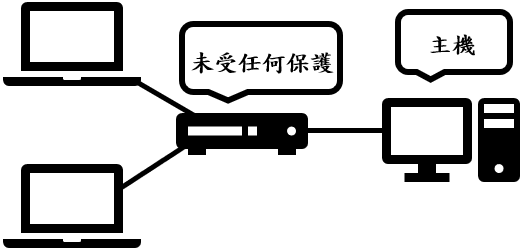
\includegraphics[width=3in]{10}
\caption{\large 普通網路}\label{fig.普通網路}
\end{center}
\end{figure}
\par
\renewcommand{\baselinestretch}{1} %設定行距
\twelve \hspace{0.5em} Stunnel是一個可以用SSL對任意TCP連接加密的程式,並可工作在Unix和Windows平臺上。它採用Client/Server模式,將Client端的網路資料採用SSL加密後,安全的傳輸到指定的Server端再進行解密還原,然後再發送到訪問的伺服器。在加密傳輸過程中,可充分確保資料的安全性,我們只要把Server端程式安裝在局域網外的一台伺服器上,即可保證傳輸的資料在局域網內是安全的,如(圖\ref{fig.加密網路})。
\\
\par
\renewcommand{\baselinestretch}{1.7} %設定行距
\begin{figure}[hbt!]
\begin{center}
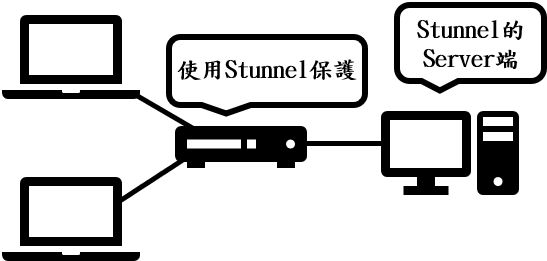
\includegraphics[width=3in]{11}
\caption{\large 加密網路}\label{fig.加密網路}
\end{center}
\end{figure}
\par
\renewcommand{\baselinestretch}{20} %設定行距
\subsection{設定操作}
\par
\renewcommand{\baselinestretch}{1} %設定行距
\twelve \qquad 因為要將Fossil採用HTTPS內容與Stunnel互動。因此與Stunnel HTTPS結合,此外需要將stunnel.conf設定如下。
\\
\par
\begin{center}
\begin{tabular}{||p{15cm}|} %表格
\hline
[https]
\\
accept = pj5073.cycu.org:443
\\
connect = 9000
\\
cert = fullchain.pem
\\
key = privkey.pem
\\
TIMEOUTclose = 0
\\
\hline
\end{tabular}
\end{center}
\clearpage %換頁
\par
\renewcommand{\baselinestretch}{1} %設定行距
\twelve \hspace{0.5em} 原本使用的cert與key是使用localhost.crt與localhost.key為自簽章憑證,自簽章憑證一樣可以用來加密,但是由於該憑證不屬於公開金鑰基礎建設簽發憑證,其他沒信任該憑證的HTTPS存取者的網頁瀏覽器會顯示一個警告,說這個憑證不被他們的電腦或瀏覽器信任。因此必須接受數位簽章的public key,因此cert與key目前已經設定為public key,此部分由後續的3.6 Let's Encrypt章節所探討。
\par
\renewcommand{\baselinestretch}{20} %設定行距
\subsection{負載平衡}
\par
\renewcommand{\baselinestretch}{1} %設定行距
\twelve \qquad 用來在多個電腦、網路連接、CPU、磁碟驅動器或其他資源中分配負載,以達到最佳化資源使用、最大化吞吐率、最小化回應時間、同時避免過載的目的。使用帶有負載平衡的多個伺服器組件,取代單一的組件,可以通過冗餘提高可靠性。
\\
\par
\renewcommand{\baselinestretch}{1} %設定行距
\twelve \hspace{0.5em} 利用Stunnel將本地服務器的IP地址與端口port 9000、5000、5001、9001的資訊,分別轉給外部的客戶端連接端口443、8443、9443、5443的HTTPS協定連線,設定如下。

\par
\begin{center}
\begin{tabular}{||p{15cm}|} %表格
\hline
[https]
\\
accept  = pj5073.cycu.org:443
\\
connect = 9000
\\
cert = fullchain.pem
\\
key = privkey.pem
\\
TIMEOUTclose = 0
\\
\\ 
[https]
\\
accept = pj5073.cycu.org:8443
\\
connect = 5000
\\
cert = fullchain.pem
\\
key = privkey.pem
\\
TIMEOUTclose = 0
\\
\\
[https]
\\
accept = pj5073.cycu.org:9443
\\
connect = 5001
\\
cert = fullchain.pem
\\
key = privkey.pem
\\
TIMEOUTclose = 0
\\
\\
[https]
\\
accept = pj5073.cycu.org:5443
\\
connect = 9001
\\
cert = fullchain.pem
\\
key = privkey.pem
\\
TIMEOUTclose = 0
\\
\hline
\end{tabular}
\end{center}
\par

\renewcommand{\baselinestretch}{20} %設定行距
\section{Nginx}
\par
\renewcommand{\baselinestretch}{1} %設定行距
\twelve \qquad 
\par}

\section{NSSM}
\par
\renewcommand{\baselinestretch}{1} %設定行距
\twelve \qquad 
\par}

\section{Let's Encrypt}
\par
\renewcommand{\baselinestretch}{1} %設定行距
\twelve \qquad 
\par}

